\documentclass{article}
\usepackage{hyperref}
\usepackage{listings}
\usepackage{color}
\usepackage{xcolor}
\usepackage{geometry}
\usepackage{graphicx}
\usepackage{amsmath}
\usepackage{caption}
\usepackage{subcaption}
\usepackage[capitalise]{cleveref}
\usepackage{wrapfig}
\usepackage{amssymb}

\geometry{margin=1in}
\pdfminorversion=6

\newcommand\TODO[1]{\textcolor{red}{TODO: #1}}

\newcommand\header[2]{
    \begin{center}
        {\large
        UCSD CSE 167 Assignment #1: \\
        \vspace{0.3cm}
        \Large
        #2}
    \end{center}
}

\definecolor{dkgreen}{rgb}{0,0.6,0}
\definecolor{gray}{rgb}{0.5,0.5,0.5}
\definecolor{mauve}{rgb}{0.58,0,0.82}
\lstset{frame=tb,
        aboveskip=3mm,
        belowskip=3mm,
        showstringspaces=false,
        columns=flexible,
        basicstyle={\small\ttfamily},
        numbers=none,
        numberstyle=\tiny\color{gray},
        keywordstyle=\color{blue},
        commentstyle=\color{dkgreen},
        stringstyle=\color{mauve},
        breaklines=true,
        breakatwhitespace=true,
        tabsize=2
}

\lstdefinelanguage{Slang}{
  sensitive=true,
  morekeywords=[1]{
    if,else,for,while,do,switch,case,default,
    break,continue,return,discard,
    struct,class,interface,enum,
    static,const,uniform,
    in,out,inout,
    import,module,
    let,var
  },
  morekeywords=[2]{
    void,bool,
    int,int2,int3,int4,
    uint,uint2,uint3,uint4,
    float,float2,float3,float4,
    half,half2,half3,half4,
    float2x2,float3x3,float4x4,
    StructuredBuffer,RWStructuredBuffer,
    ByteAddressBuffer,RWByteAddressBuffer,
    Texture1D,Texture2D,Texture3D,TextureCube,
    RWTexture1D,RWTexture2D,RWTexture3D,
    SamplerState
  },
  morekeywords=[3]{
    shader,numthreads,
    SV_DispatchThreadID,SV_GroupID,SV_GroupThreadID,
    SV_Position,SV_Target,
    dot,cross,length,normalize,
    mul,lerp,clamp,saturate,
    min,max,abs,sqrt,pow,
    sin,cos,tan,asin,acos,atan,
    floor,ceil,round,frac,
    reflect,refract
  },
  morecomment=[l]{//},
  morecomment=[s]{/*}{*/},
  morestring=[b]"
}

\lstdefinestyle{slang}{
  language=Slang,
  basicstyle=\ttfamily\small,
  keywordstyle=[1]\color{blue},
  keywordstyle=[2]\color{teal},
  keywordstyle=[3]\color{violet},
  commentstyle=\color{gray},
  stringstyle=\color{orange},
  showstringspaces=false,
  columns=fullflexible,
  keepspaces=true,
  breaklines=true
}

% Taken from https://tex.stackexchange.com/questions/83085/how-to-improve-listings-display-of-json-files

\colorlet{punct}{red!60!black}
\definecolor{delim}{RGB}{20,105,176}
\colorlet{numb}{magenta!60!black}

\lstdefinelanguage{json}{
    basicstyle=\normalfont\ttfamily,
    numberstyle=\scriptsize,
    stepnumber=1,
    numbersep=8pt,
    showstringspaces=false,
    breaklines=true,
    frame=lines,
    tabsize=2,
    literate=
     *{0}{{{\color{numb}0}}}{1}
      {1}{{{\color{numb}1}}}{1}
      {2}{{{\color{numb}2}}}{1}
      {3}{{{\color{numb}3}}}{1}
      {4}{{{\color{numb}4}}}{1}
      {5}{{{\color{numb}5}}}{1}
      {6}{{{\color{numb}6}}}{1}
      {7}{{{\color{numb}7}}}{1}
      {8}{{{\color{numb}8}}}{1}
      {9}{{{\color{numb}9}}}{1}
      {:}{{{\color{punct}{:}}}}{1}
      {,}{{{\color{punct}{,}}}}{1}
      {\{}{{{\color{delim}{\{}}}}{1}
      {\}}{{{\color{delim}{\}}}}}{1}
      {[}{{{\color{delim}{[}}}}{1}
      {]}{{{\color{delim}{]}}}}{1},
}

\hypersetup{colorlinks=true}


\begin{document}

\header{1}{2D Graphics}
\setcounter{section}{-1}

Computer graphics is the field that studies how to process \emph{visual data}, such as shapes, volumes, and lights. \textbf{Images} are an important class of visual data: they can be the pictures recorded by the camera of your cellphone or a DSLR, outputs of video games or movie visual effects, legends and arrows on Google map telling you where to go next, or visualization of the radio waves coming from a black hole. An important subfield of computer graphics, rendering, studies the generation of images.

\begin{figure}[h]
    \centering
    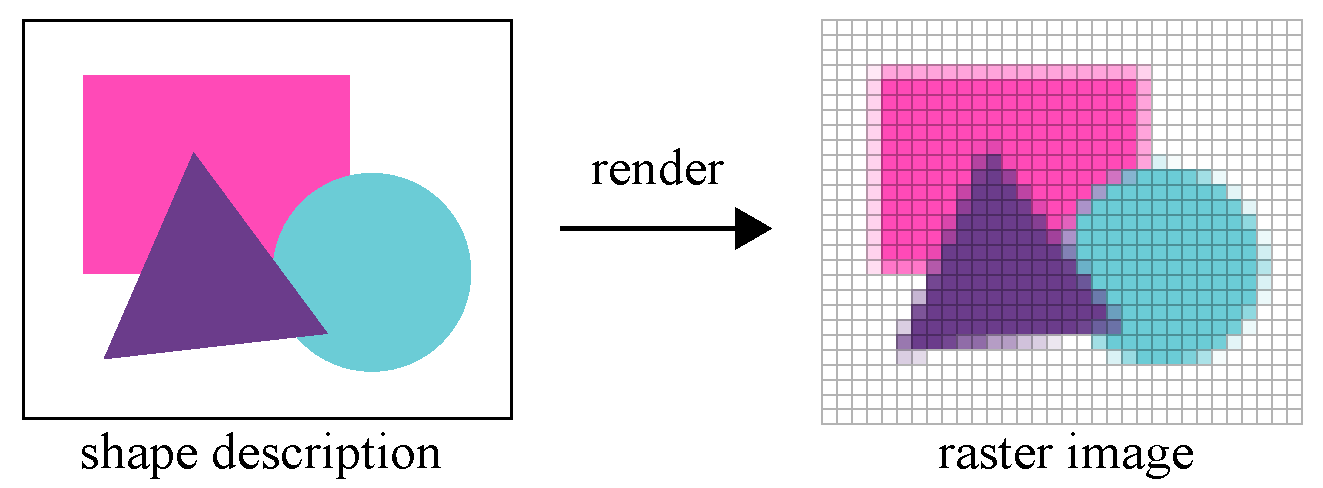
\includegraphics[width=0.6\linewidth]{imgs/render2d.pdf}
    \caption{In this homework, we will render a set of 2D shapes into a raster image.}
    \label{fig:render2d}
\end{figure}

In our first homework, we will implement a 2D renderer that takes ``shapes'' (e.g., circle, lines, squares, and triangles), and turn them into a raster image (\cref{fig:render2d}). A raster image is a particular kind of image that represent 2D contents using a grid of \emph{pixels}, where each pixel denotes the color at that location. Raster images are convenient because our displays (and our camera sensor) usually also represent images as a grid of pixels.

Before you start coding, we recommend you to go through the whole handout to have some ideas of what needs to be done. Some of the instructions are \textbf{intentionally vague} because we want you to figure things out. Please come to our office hours or ask on Piazza if you have any questions.

\paragraph{Submission.} Submit your code and the outputs of your code through Canvas. Please zip them without the temporary object files and binaries generated by the compiler.

\paragraph{Grading.} We will compare your outputs to our reference solutions. You don't have to be accurate at binary level (as there will be floating point cancellation errors), we allow some error margins (the TAs will check manually if something seems off).

\paragraph{Collaboration policy.} We allow a team up to two people. The homeworks are pretty dense and time-consuming (much harder than last year!), so we encourage you to team up. You can solo too if you want.

\paragraph{In-person code interview.} After submitting the homework, each team will do
a short interview during the Discussion section on Friday 3pm (right after the lecture). This will usually take around a minute or two (this is a big class so we need to be efficient). 
Both group members should attend, and either can answer the questions.
We may ask you to explain a part of
your implementation, predict what the code will do if we change something, or ask you
to modify the code in a particular way. Some teams may get additional follow-up questions.

The interview acts as a multiplier on your homework grade. Normally the multiplier
is 1. Minor mistakes, nervousness, or forgetting syntax will not reduce your grade.
If you have substantial difficulty explaining your code, we may ask more questions or do a longer follow-up.
The multiplier will be reduced in serious cases after follow-up.

If you cannot come to the discussion session, come to our office hours.
(Missing the interview results in a multiplier of 0.)

We are not testing whether you memorized Slang/Python syntax. We want to make sure
you have an operational understanding of what your renderer is doing.

\paragraph{Language models policy.} We do not encourage heavily using language models
for your homeworks. Figuring out how to do things yourself is an important part of learning
process. Treat language models as TAs/tutors: you can ask them questions, but you should
not let them code for you. Maybe try coming to us first? 

Using language models for installing balboa/slangpy is acceptable (maybe even encouraged). 
In general, if you think more as a result of using language models, it's probably fine. 
If you use it to save time or think less, it's often not fine.

If you used language models, you should report your usage in detail (saying "I used ChatGPT to help" is not sufficient).

Our homework problems roughly build on one another: homework 1.2 will be based on homework 1.1, and 1.3 will be based on 1.2, and so on. Feel free to start by copy pasting your previous solution if you feel it will be useful. (That's what I did.)

\section{Balboa and slangpy}
We are going to build our code on top of a currently barebone codebase \emph{balboa}. Balboa is a Python codebase, so all you need to do is
\begin{lstlisting}[language=bash]
  git clone https://github.com/BachiLi/balboa_slang_public
\end{lstlisting}
Balboa uses \lstinline{uv} to manage its Python dependencies. 
Read the \href{https://docs.astral.sh/uv/getting-started/installation/}{installation guide} to figure out how to install uv on your system.
When you are in the Balboa directory, run
\begin{lstlisting}[language=bash]
  uv sync
\end{lstlisting}

The most important dependency is \href{https://github.com/shader-slang/slangpy}{slangpy}, which will be the GPU framework we use throughout the course.

Once you have done with these, run
\begin{lstlisting}[language=bash]
  uv run python main.py 1_1
\end{lstlisting}
(\lstinline{1_1} means homework 1.1). You should see a GUI window with a white background.

\section{Rendering a single circle (5 pts)}

\begin{figure}[h]
    \centering
    \begin{subfigure}[t]{0.4\linewidth}
        \centering
        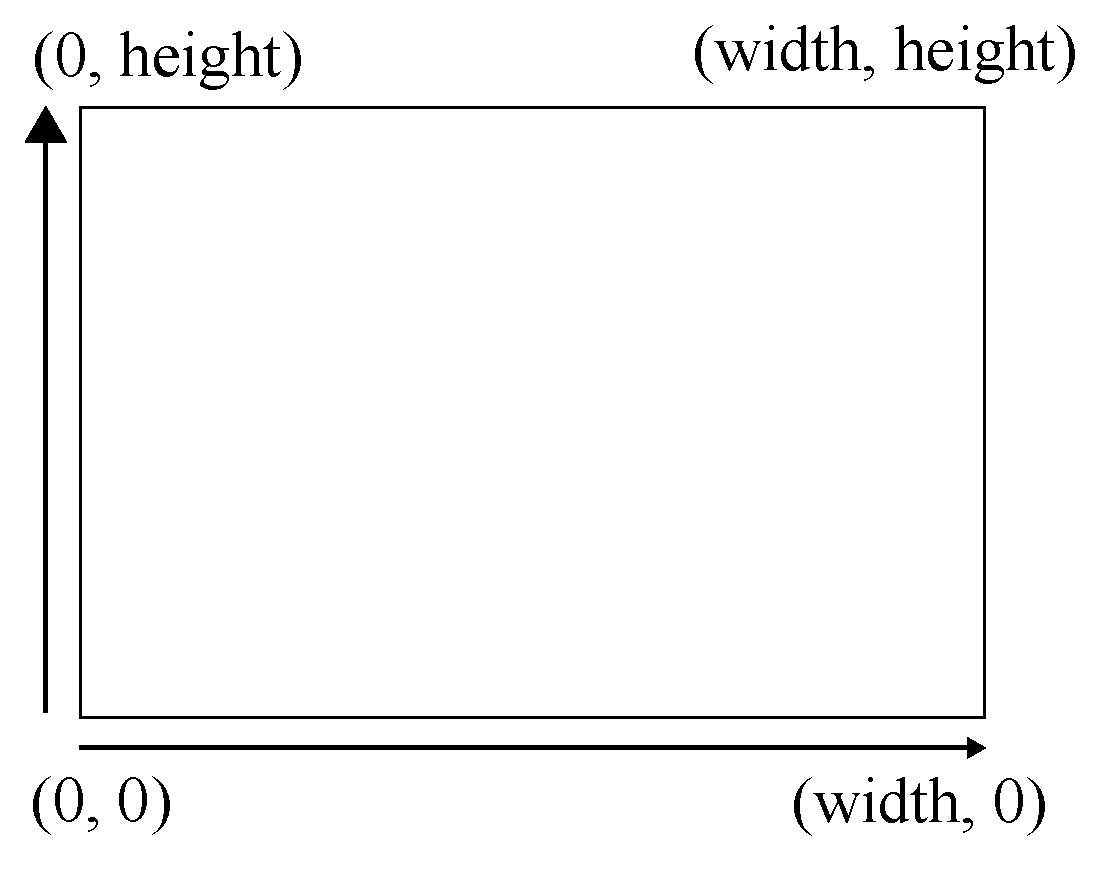
\includegraphics[width=\linewidth]{imgs/canvas.pdf}
        \caption{\label{fig:canvas}}
    \end{subfigure}
    \begin{subfigure}[t]{0.4\linewidth}
        \centering
        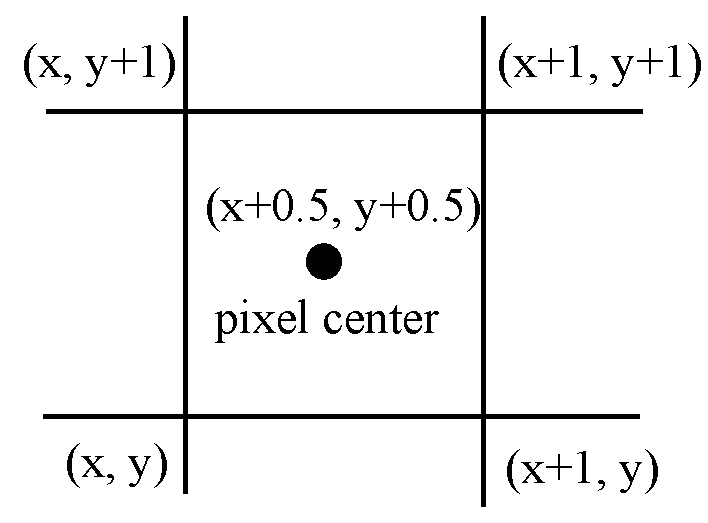
\includegraphics[width=\linewidth]{imgs/pixel.pdf}
        \caption{\label{fig:pixel}}
    \end{subfigure}
    \caption{(a) The coordinate system of the ``canvas'' we will draw our shapes on. (b) The pixel center of for pixel $(x, y)$ locates at $(x+0.5, y+0.5)$.}
\end{figure}

In the first part of this homework, we will render a single circle on our image. We are given a gray ``canvas'', where in this part we assume it to be of size $640 \times 480$. We need a \textbf{coordinate system} to talk about points on this canvas -- \cref{fig:canvas} illustrates the coordinate system. We call this coordinate system the ``screen space''.
We are further given the center, radius, and color of the circle. These are command line arguments that we will parse for you.

To render an image, we need to determine the color for each pixel. For this part, we focus on determining the color of the center of the pixel (\cref{fig:pixel}). To determine the pixel color, we decide whether the pixel center hits the circle or not. If it hits the circle, then we decide that the pixel's color is the circle's color. Otherwise, we decide that the pixel's color is the background color (by default, let's say it's $(0.5, 0.5, 0.5)$). How to decide whether the pixel center hits the circle? That's for you to figure out!

\paragraph{Compute shaders.}
You'll write your code inside a GPU \emph{shader}. A shader is a parallel GPU program that launches many threads simultaneously to draw a picture. We choose the Slang language for implementing shaders: it's cross platform and it is very similar to popular languages like HLSL. Look at \lstinline{hw1/hw1_1.slang} and you will see the following code:
\begin{lstlisting}[language=Slang]
[shader("compute")]
[numthreads(8, 8, 1)]
void compute_main(uint2 tid : SV_DispatchThreadID,
                  uniform float2 center,
                  uniform float radius,
                  uniform float3 color,
                  RWTexture2D<float4> image) {
    uint width, height;
    image.GetDimensions(width, height);
    if (tid.x >= width || tid.y >= height) {
        return;
    }
    image[tid] = float4(1.0);
    // TODO: your code here
}
\end{lstlisting}

Let's look at the code line-by-line:
\begin{lstlisting}[language=Slang]
[shader("compute")]
\end{lstlisting}
means that this is a \emph{compute shader}. Compute shaders are general-purpose GPU programs that can perform general computation.
For now, knowing that a compute shader launches many threads in parallel is sufficient.
\begin{lstlisting}[language=Slang]
[numthreads(8, 8, 1)]
\end{lstlisting}
means that the parallel threads we launched are organized into 2D groups of $8 \times 8=64$ threads. 
GPU execute threads in small groups called \emph{warps} or \emph{waves}, typically containing $32$ or $64$ threads,
so using $64$ threads per thread group is a reasonable choice on current GPUs.

The total number of threads launched is specified outside in the CPU code. If we want to process a $31 \times 23$ image, for example,
balboa uses SlangPy to launch $4 \times 3$ groups of $8 \times 8$ threads. Therefore we are actually launching $32 \times 24$ threads.
\begin{lstlisting}[language=Slang]
void compute_main(uint2 tid : SV_DispatchThreadID,
\end{lstlisting}
\lstinline{compute_main} is our entry point, and \lstinline{tid} is a 2D unsigned integer vector that represents our current 2D global thread ID.
\begin{lstlisting}[language=Slang]
          uniform float2 center,
          uniform float radius,
          uniform float3 color,
\end{lstlisting}
these are our parameters for the circle and its color. The specifier \lstinline{uniform} means that these parameters have the same values across threads. All the threads see the same \lstinline{center} parameter, for example.
\begin{lstlisting}[language=Slang]
          RWTexture2D<float4> image) {
\end{lstlisting}
This is our output. Our image is defined as a 2D texture that is both readable and writable (RW). Each pixel stores a \lstinline{float4}, which we interpret as red, green, blue, and alpha (RGBA). Alpha here is related to opacity, which will make more sense when we get to alpha blending later.
\begin{lstlisting}[language=Slang]
    uint width, height;
    image.GetDimensions(width, height);
\end{lstlisting}
This gives us the size of the image.
\begin{lstlisting}[language=Slang]
    if (tid.x >= width || tid.y >= height) {
        return;
    }
\end{lstlisting}
As mentioned earlier, the launched number of threads will be multiple of $8$ at each dimension. Meanwhile our image may not have width and height to be multiples of $8$. So we need to guard the threads that ``overflow''.

Finally,
\begin{lstlisting}[language=Slang]
	image[tid] = float4(1.0);
\end{lstlisting}
This writes white color to the image pixel corresponding to our current 2D thread ID.

\paragraph{Slang shading language and vector math.} 
The shading language is very C-like, so if you have written C or C++ before it should look familiar. The Slang shading language, which itself borrows heavily from HLSL, has some built-in support for common vector and linear algebra operations. You have seen \lstinline{float2} and \lstinline{float3}. Here are some things you can do with them:
\begin{lstlisting}[language=Slang]
float2 p = float2(1.0, 2.0);
float2 q = float2(3.0, 4.0);
float3 c = float3(1.0, 0.5, 0.2);
float4 rgba = float4(c, 1.0);

p.x
p.y
c.xy // returns float2
rgba.xyz // returns float3
rgba.zxy // returns float3

p + q
2.0 * p
p / 3.0

dot(p, q)
length(p)
normalize(p)

// matrix vector multiplication
float3 Mp = mul(M, float3(p, 1.0));

float x = p[0];
\end{lstlisting}
See \href{https://docs.shader-slang.org/en/stable/external/slang/docs/language-reference/types-vector-and-matrix.html}{this page} for more information.

Here are some commonly used math functions
\begin{lstlisting}[language=Slang]
abs(x)
min(x, y)
max(x, y)
clamp(x, min, max)
sqrt(x)
sin(x)
cos(x)
acos(x)
dot(x, y)
length(x)
normalize(x)
lerp(x, y, s) // linear interpolation
\end{lstlisting}
Check out \href{https://learn.microsoft.com/en-us/windows/win32/direct3dhlsl/dx-graphics-hlsl-intrinsic-functions}{this page} for a comprehensive list, though you likely only need the ones above.

You should be ready to implement the circle rendering code in \lstinline{hw1/hw1_1.slang} at this point. 
To see your results, in terminal, type:
\begin{lstlisting}[language=bash]
  uv run python main.py 1_1 -center 200 300 -radius 100 -color 0.3 0.7 0.5
  uv run python main.py 1_1 -center -50 250 -radius 100 -color 0.7 0.3 0.3
  uv run python main.py 1_1 -center 600 250 -radius 150 -color 0.3 0.5 0.7
  uv run python main.py 1_1 -center 250 470 -radius 50 -color 0.7 0.5 0.7
\end{lstlisting}
or just any parameter you like! \cref{fig:hw1_1} shows our rendering for the first command.

In your submission, save the image generated by the following special commands that skip the GUI:
\begin{lstlisting}[language=bash]
  uv run python main.py -output outputs/hw_1_1.png 1_1 -center -20.5 455.25 -radius 90.75 -color 0.7 0.5 0.7
\end{lstlisting}
We will compare your output with our rendering for grading.

\begin{figure}[ht]
    \centering
    
\includegraphics[width=0.5\linewidth]{imgs/hw_1_1.png}
    \caption{Reference image for Homework 1.1.}
    \label{fig:hw1_1}
\end{figure}

If you see your circles, congratulations! If you have not done graphics-related stuff before, this is likely the first time you use code to generate an image from scratch. I still find this moment satisfying even after doing this for more than 15 years: you paint on a canvas using code (and sometimes math) instead of a brush. This makes people who are not that good in traditional art capable of generating beautiful pictures (yes, the images you generate will become prettier from now on). Furthermore, unlike things like Seedance or Veo, you maintain full control of the process: at this point, you know exactly how each pixel is generated, and if you don't like it, it's very easy to fix if you know how computer graphics works.

\section{Rendering polylines (20 pts)}
In this part, we will render a more complex shape called \href{https://developer.mozilla.org/en-US/docs/Web/SVG/Reference/Element/polyline}{polyline}, inspired by the Scalable Vector Graphics (SVG) standard. 
Therefore, what we describe below will be close to how some of the web browsers render these shapes. 
A polyline is a sequence of 2D points with straightlines connected through them. A \emph{closed} polyline means that the last point is connected to the first point.

\begin{figure}[h]
    \centering
    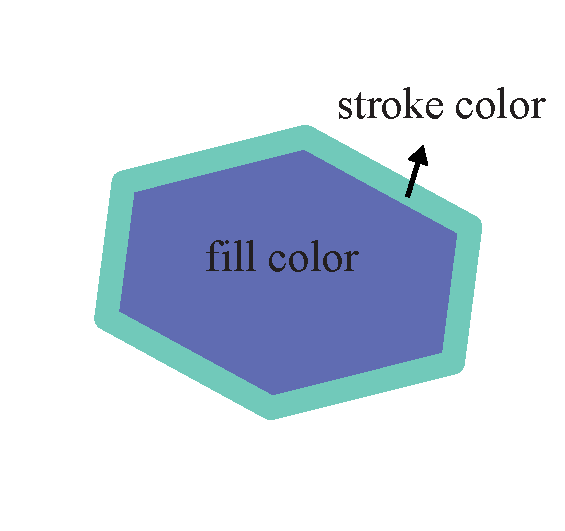
\includegraphics[width=0.3\linewidth]{imgs/fill_vs_stroke.pdf}
    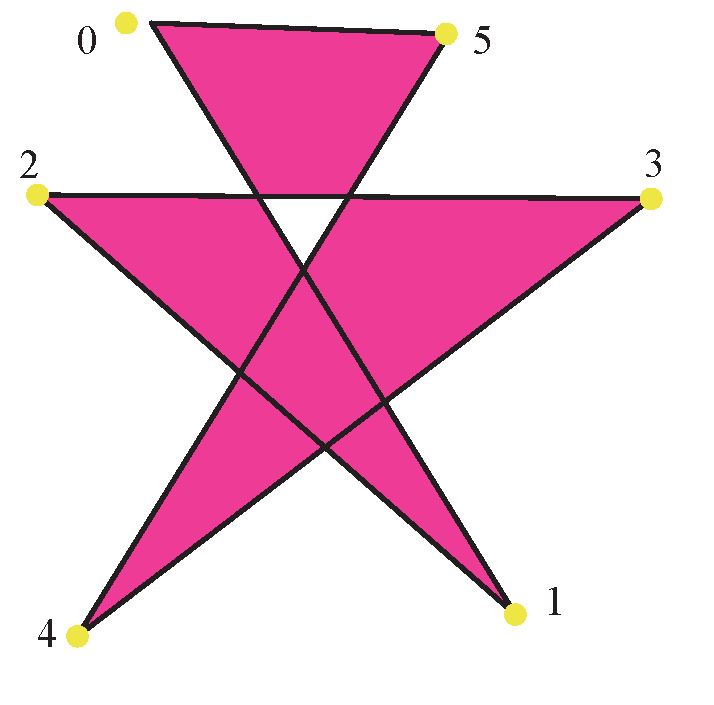
\includegraphics[width=0.3\linewidth]{imgs/fill_rule.pdf}
    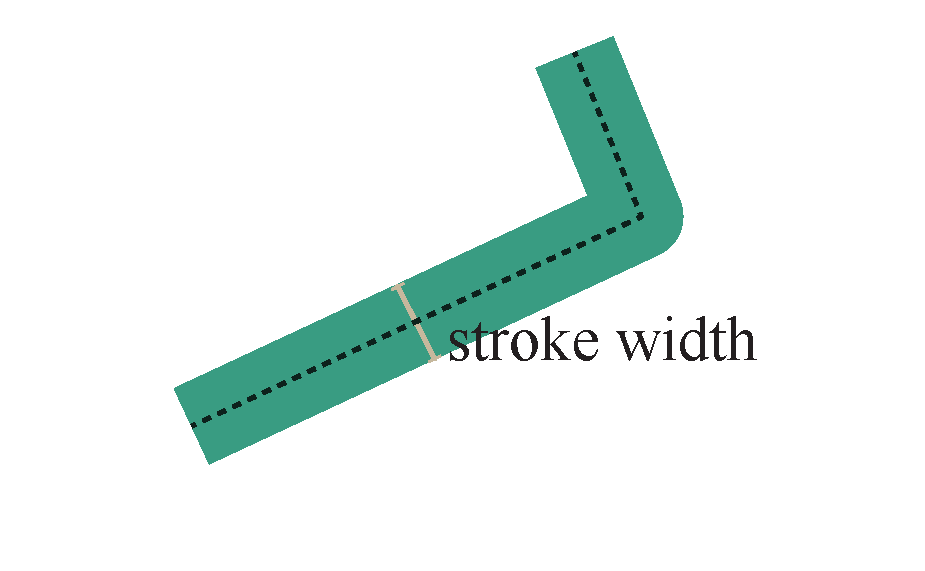
\includegraphics[width=0.3\linewidth]{imgs/stroke_width.pdf}
    \caption{(a) Fill color vs. stroke color. (b) A more complex example for fill colors (the numbers next to the points are the order). (c) Stroke width for stroke color.}
    \label{fig:fill_vs_stroke}
\end{figure}

Similar to SVG, each polyline can have a \emph{fill color} (only applies to closed polylines) and a \emph{stroke color} (applies to both open and closed polylines) defined by an additional parameter stroke width. \cref{fig:fill_vs_stroke} illustrates them (pay extra attention to a few details including the round corners of the star in \cref{fig:fill_vs_stroke}(a), the middle regions in \cref{fig:fill_vs_stroke}(b), and the flat caps of the line segment in \cref{fig:fill_vs_stroke}(c): this will give you ideas about the ordering between strokes and filled color, the filling rule of even-odd vs non-zero, and the caps rule of flat vs round). 
We should have covered how to determine whether a point belongs to fill vs stroke regions in the lectures, but it could be fun to figure it out on your own too!

\begin{figure}[ht]
    \centering
    
\includegraphics[width=0.32\linewidth]{imgs/hw_1_2a.png}
    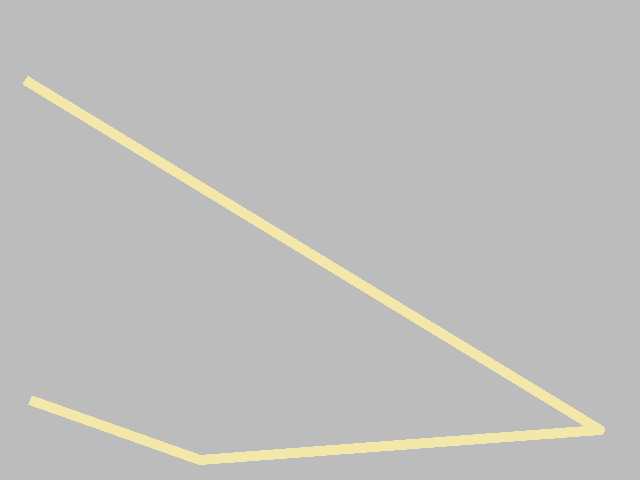
\includegraphics[width=0.32\linewidth]{imgs/hw_1_2b.png}
    
\includegraphics[width=0.32\linewidth]{imgs/hw_1_2c.png}
    \caption{References for Homework 1.2.}
    \label{fig:hw1_2}
\end{figure}

You should be able to implement the whole things in \lstinline{hw1/hw1_2.slang}. Inside, you will see the following argument:
\begin{lstlisting}[language=Slang]
          StructuredBuffer<float2> polyline,
\end{lstlisting}
A StructuredBuffer is an 1D array on GPU. You can only read from it, you cannot write into it.

To see your results, in terminal, type:
\begin{lstlisting}[language=bash]
  uv run python main.py 1_2 -points 30 30 540 200 200 400 --closed -fill_color 0.2 0.8 0.2
  uv run python main.py 1_2 -points 25 400 600 50 200 20 30 80 -stroke_color 0.9 0.8 0.4 -stroke_width 10
  uv run python main.py 1_2 -points 320 450 480 30 80 300 560 300 160 30 --closed -fill_color 0.2 0.3 0.9 -stroke_color 0.1 0.1 0.1 -stroke_width 5
\end{lstlisting}
\cref{fig:hw1_2} shows our rendering for the these three commands.

To test your code, we will use these commands:
\begin{lstlisting}[language=bash]
uv run python main.py -output outputs/hw_1_2_fill.png 1_2 -points 100 100 500 100 500 350 350 250 100 350 --closed -fill_color 0.2 0.8 0.2
uv run python main.py -output outputs/hw_1_2_caps.png 1_2 -points 150 100 500 400 -stroke_color 0.2 0.2 0.9 -stroke_width 50
uv run python main.py -output outputs/hw_1_2_joins.png 1_2 -points 250 420 300 400 200 350 450 300 150 250 500 200 100 150 550 100 320 50 320 5 -stroke_color 0.9 0.9 0.2 -stroke_width 20
uv run python main.py -output outputs/hw_1_2_fill_stroke.png 1_2 -points -40 80 420 40 570 250 260 430 30 300 --closed -fill_color 0.15 0.65 0.85 -stroke_color 0.9 0.25 0.2 -stroke_width 24
uv run python main.py -output outputs/hw_1_2_winding.png 1_2 -points 40 40 600 40 600 440 40 440 40 40 140 130 140 350 280 350 280 130 140 130 40 40 360 130 360 350 520 350 520 130 360 130 40 40 410 190 470 190 470 290 410 290 410 190 40 40 --closed -fill_color 0.9 0.4 0.2
\end{lstlisting}
We will compare your renderings with ours. Each rendering is worth 4 points.

\section{Rendering multiple shapes (10 pts)}

Next, we will add the ability of rendering multiple shapes in our renderer. Before that, let's introduce our scene file format, so that we can easily create new scenes. There is no single standard way to represent a scene in computer graphics.\footnote{Though in 2D, \href{https://en.wikipedia.org/wiki/SVG}{Scalable Vector Graphics (SVG)} is the most popular, and in 3D, studios are converging towards the \href{https://en.wikipedia.org/wiki/Universal_Scene_Description}{Universal Scene Description}.} Thus, we will use an easily readable and parsable \href{https://en.wikipedia.org/wiki/JSON}{JSON} format to describe our scene. It's easiest to explain by directly showing a scene:
\begin{lstlisting}[language=json]
{
    "resolution": [640, 360],
    "background": [
        0.4, 0.6, 0.4
    ],
    "objects": [
        {
            "type": "circle",
            "center": [320, 180],
            "radius": 160,
            "fill_rgba": [0.1, 0.3, 0.95, 1.0]
        },
        {
            "type": "circle",
            "center": [150, 280],
            "radius": 80,
            "stroke_rgba": [0.95, 0.1, 0.3, 1.0],
            "stroke_width": 10
        },
        {
            "type": "circle",
            "center": [490, 280],
            "radius": 80,
            "fill_rgba": [0.95, 0.1, 0.3, 1.0]
        }
    ]
}
\end{lstlisting}
\begin{figure}[ht]
    \centering
    
\includegraphics[width=0.45\linewidth]{imgs/hw_1_3a.png}
    
\includegraphics[width=0.45\linewidth]{imgs/hw_1_3b.png}
    \caption{References for Homework 1.3.}
    \label{fig:hw1_3}
\end{figure}
The corresponding image is at the left of \cref{fig:hw1_3} (pay attention to the detail of the ordering of the shapes).

We will provide the scene parser for you. The scene is parsed and transformed into the following Slang data structures:
\begin{lstlisting}[language=Slang]
// Common scene definitions
enum ShapeType {
    Circle,
    Polyline,
    QuadraticBezier
};

struct Shape {
    ShapeType type;
    // where the shapes is in circles/polylines arrays
    int index;

    bool use_fill;
    float4 fill_rgba;
    bool use_stroke;
    float4 stroke_rgba;
    float stroke_width;
    float3x3 world_to_obj;
};

struct Circle {
    float2 center;
    float radius;
};

struct Polyline {
    int pts_begin; // starting location in the points array
    int pts_end; // end location in the points array
    bool closed;
};

struct QuadraticBezier {
    int pts_begin;
    int pts_end;
    bool closed;
};
\end{lstlisting}
Don't worry about the QuadraticBezier for now. 

In \lstinline{hw1_3.slang}, you receive the scene directly in the function arguments:
\begin{lstlisting}[language=Slang]
void main(uint2 tid : SV_DispatchThreadID,
          uniform float3 background,
          uniform int /*samples_per_axis*/, // ignore for now
          StructuredBuffer<Shape> shapes,
          StructuredBuffer<Circle> circles,
          StructuredBuffer<Polyline> polylines,
          StructuredBuffer<QuadraticBezier> /*quadratic_beziers*/, // ignore for now
          StructuredBuffer<float2> points,
          RWTexture2D<float4> image) {
\end{lstlisting}

For \lstinline{Polyline}, we consolidate all of their points inside the \lstinline{points} array, and store indices inside the \lstinline{Polyline} struct. This is a common trick to flatten hierarchical data structures on GPU, giving us contiguous storage and GPU-friendly memory access

Our JSON scenes support (axis-aligned) rectangles and triangles, but they are converted to polylines by our scene parser, so handling circles and polylines should be sufficient for this subproblem.

Write your code in \lstinline{hw1/hw1_3.slang} and test it using the following commands:
\begin{lstlisting}[language=bash]
  uv run python main.py 1_3 scenes/hw1/four_circles.json
  uv run python main.py 1_3 scenes/hw1/four_shapes.json
\end{lstlisting}

We show our rendering of the two scenes in \cref{fig:hw1_3}.
We will grade your results using the following scenes:
\begin{lstlisting}[language=bash]
  uv run python main.py -output outputs/hw_1_3_many_shapes.png 1_3 scenes/hw1/many_shapes.json
  uv run python main.py -output outputs/hw_1_3_cat.png 1_3 scenes/hw1/cat.json
\end{lstlisting}

I also made this robot for you to render yourself.
\begin{lstlisting}[language=bash]
  uv run python main.py 1_3 scenes/hw1/robot.json
\end{lstlisting}

\section{2D transformation (15 pts)}

Next, we're going to edit our shapes using some 2D transformations. These transformations can help us render more interesting shapes and generate animations. We are going to focus on \emph{affine} transformations, where each point $x \in \mathbb{R}^2$ in the shape is transformed through the expression $Ax + b$ where $A$ is some $2 \times 2$ matrix and $b$ is a 2D vector. 

\begin{figure}[t]
    \begin{subfigure}[t]{0.195\linewidth}
        \centering
        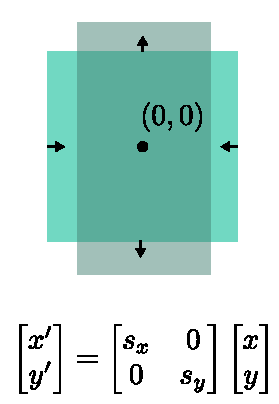
\includegraphics[width=\linewidth]{imgs/scale.pdf}
        \caption{\label{fig:scale} scale}
    \end{subfigure}
    \begin{subfigure}[t]{0.195\linewidth}
        \centering
        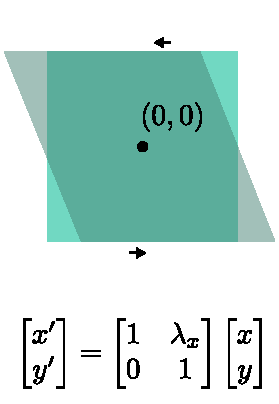
\includegraphics[width=\linewidth]{imgs/shear_x.pdf}
        \caption{\label{fig:shear_x} shear x}
    \end{subfigure}
    \begin{subfigure}[t]{0.195\linewidth}
        \centering
        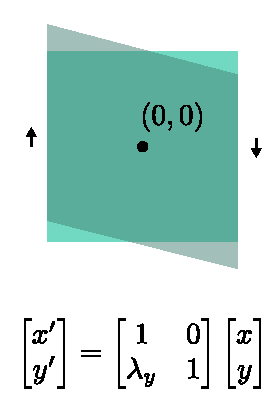
\includegraphics[width=\linewidth]{imgs/shear_y.pdf}
        \caption{\label{fig:shear_y} shear y}
    \end{subfigure}
    \begin{subfigure}[t]{0.195\linewidth}
        \centering
        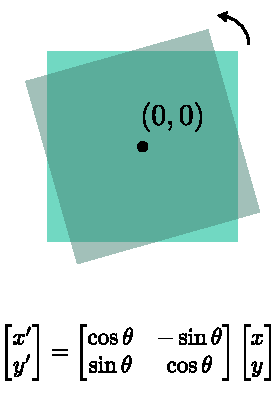
\includegraphics[width=\linewidth]{imgs/rotate.pdf}
        \caption{\label{fig:rotate} rotate}
    \end{subfigure}
    \begin{subfigure}[t]{0.195\linewidth}
        \centering
        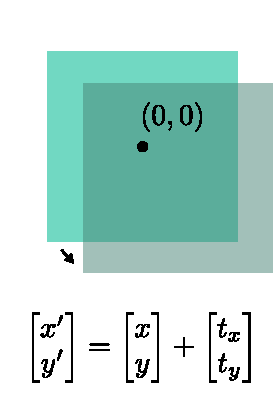
\includegraphics[width=\linewidth]{imgs/translate.pdf}
        \caption{\label{fig:translate} translate}
    \end{subfigure}
    \caption{\label{fig:transformation} The five affine transformations we will support in this homework. Here we assume x axis is pointing right and y axis is pointing up. Notice that only the translation cannot be expressed using a $2 \times 2$ matrix.}
\end{figure}

\begin{figure}[t]
    \begin{subfigure}[t]{0.195\linewidth}
        \centering
        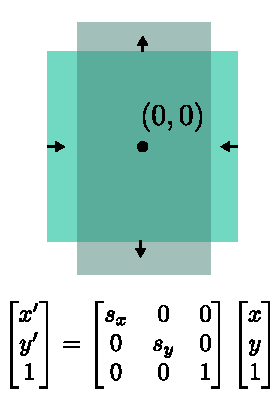
\includegraphics[width=\linewidth]{imgs/scale_affine.pdf}
        \caption{\label{fig:scale_affine} scale}
    \end{subfigure}
    \begin{subfigure}[t]{0.195\linewidth}
        \centering
        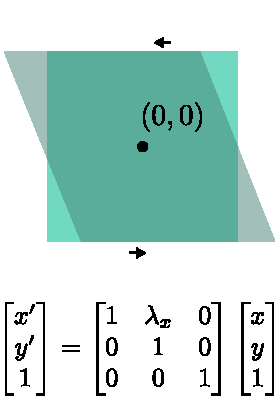
\includegraphics[width=\linewidth]{imgs/shear_x_affine.pdf}
        \caption{\label{fig:shear_x_affine} shear x}
    \end{subfigure}
    \begin{subfigure}[t]{0.195\linewidth}
        \centering
        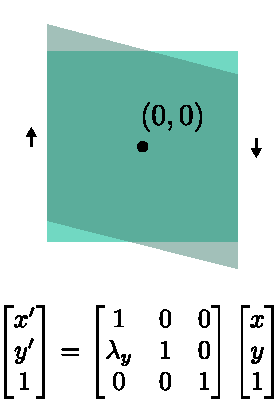
\includegraphics[width=\linewidth]{imgs/shear_y_affine.pdf}
        \caption{\label{fig:shear_y_affine} shear y}
    \end{subfigure}
    \begin{subfigure}[t]{0.195\linewidth}
        \centering
        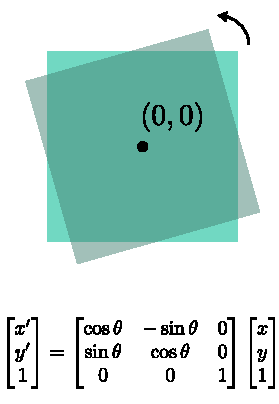
\includegraphics[width=\linewidth]{imgs/rotate_affine.pdf}
        \caption{\label{fig:rotate_affine} rotate}
    \end{subfigure}
    \begin{subfigure}[t]{0.195\linewidth}
        \centering
        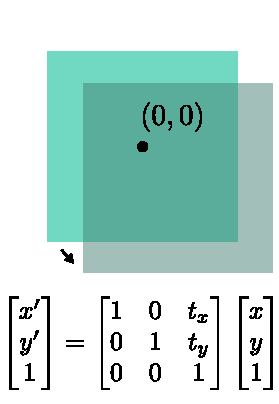
\includegraphics[width=\linewidth]{imgs/translate_affine.pdf}
        \caption{\label{fig:translate_affine} translate}
    \end{subfigure}
    \caption{\label{fig:transformation_affine} Using \emph{augmented matrices}, we can represent all affine transforms, including translation, using $3 \times 3$ matrices. We recommend you to hand compute these matrix vector products and confirm they are the same as \cref{fig:transformation}.}
\end{figure}

In this part, we will implement a few common affine transformations: scaling, shearing, rotation, and translation (in fact, all affine transformations can be written as combinations of these transformations, see ``polar decomposition'' if you are interested). Crucially, we also want to \emph{combine} these transformations: for example, we might want to first rotate the shape, then translate it. As noted in \cref{fig:transformation}, everything except for translation can be represented as a matrix-vector product. This is annoying for combining the transformations: for all other transformations, we can combine them by multiplying the transformation matrices: for example, if we want to first rotate using matrix $R$ then scale using matrix $S$, we can combine them into a single matrix $S R$ (think: why isn't it $R S$?). The existence of translation makes this difficult. Fortunately, there is a very clever trick to unify every affine transformation into matrix vector products: observe that
\begin{equation}
\begin{bmatrix}
x' \\ y' \\ 1
\end{bmatrix}
=
\begin{bmatrix}
a_{00} & a_{01} & b_{0} \\
a_{10} & a_{11} & b_{1} \\
0 & 0 & 1
\end{bmatrix}
\begin{bmatrix}
x \\ y \\ 1
\end{bmatrix}
\end{equation}
is equivalent to
\begin{equation}
\begin{bmatrix}
x' \\ y'
\end{bmatrix}
=
\begin{bmatrix}
a_{00} & a_{01} \\
a_{10} & a_{11}
\end{bmatrix}
\begin{bmatrix}
x \\ y
\end{bmatrix}
+
\begin{bmatrix}
b_0 \\ b_1
\end{bmatrix}
\end{equation}

Therefore, we can represent all affine transformations using the $3 \times 3$ matrix above. \cref{fig:transformation_affine} shows the corresponding version of the matrices for each transformation.

Another cool feature about augmented matrices is that they allow us to distinguish between \emph{points} and \emph{vectors}. For points, we set the third component to be $1$. For vectors, we set the third component to be $0$. This allows us to \emph{turn off} translation for vectors: translating a vector should not affect its values! 

To describe affine transformations in our scene files, for each object, we can have a \lstinline{transform} property:
\begin{lstlisting}[language=json]
{
    "type": "circle",
    "fill_rgba": [0.3, 0.5, 0.8, 1.0],
    "transform": [
        {"scale": [200, 100]},
        {"rotate": [45]},
        {"translate": [320, 180]}
    ]
}
\end{lstlisting}
(Note that the rotation is described in degrees, not radians.)
The circle has the default radius ($1$) and center ($(0, 0)$). The transformations are applied in the order they appear: the circle is first scaled, then rotated, then translated (think: how would it look like?). Mathematically, if we denote the scaling matrix as $S$, the rotation matrix as $R$, and translation matrix as $T$, then the affine transformation matrix $F$ is:
\begin{equation}
    \text{translate}(\text{rotate}(\text{scale}(x))) = T R S x = F x
\end{equation}
The affine transformation matrix allows us to easily chain these operations and store the final result in a single matrix $F$.

\begin{figure}[ht]
    \centering
    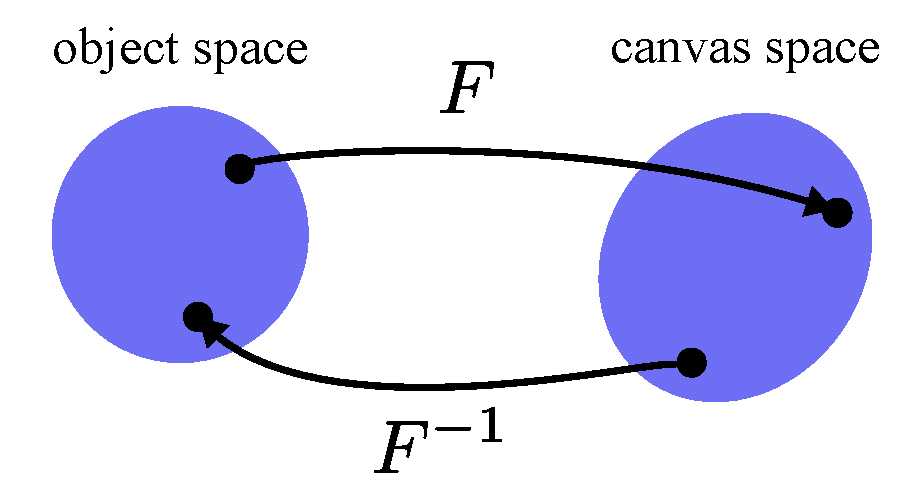
\includegraphics[width=0.5\linewidth]{imgs/spaces.pdf}
    \caption{Transformation converts points between spaces.}
    \label{fig:spaces}
\end{figure}

The transformation matrix above can be seen as a relation between \emph{spaces}. We call the space before the transformation the \emph{object space} because this is where the space the original object is described in. Here, the transformation (let's call it $F$) converts points in the object space to the \emph{screen space}. On the other hand, the \emph{inverse} of the transformation $F^{-1}$ (i.e., matrix inversion) converts points in the screen space to the object space. See \cref{fig:spaces} for a visualization.

The remaining question we need to address is: how do we test if the pixel center has hit the transformed shape? A main challenge is that the transformed shape may not be as easy to test compared to the original shape. For example, after linear transformations, a circle may become an ellipse. The trick we are going to test in the object space, instead of the screen space. Given a screen space point $x$ representing a pixel's center, we convert it to the object space using the inverse transform $F^{-1}$, then test whether it hits the object after the inverse transform. 

To complete your implementation, first go to \lstinline{hw1/hw1_scenes.py} and complete the function \lstinline{compose_transformation}: this function parses the sequence of transformations and combines them into a $3 \times 3$ matrix, which by default will be a matrix that transforms from object space to world space.
After that, the matrix is inverted in \lstinline{upload_scene} which I have implemented.
The resulting transformation will store in the \lstinline{world_to_obj} member of the \lstinline{Shape} struct. Next, go to \lstinline{hw1/hw1_4.slang} and finish your implementation to render transformed shapes.

Test your rendering using the following commands:
\begin{lstlisting}[language=bash]
  uv run python main.py 1_4 scenes/hw1/transformation.json
\end{lstlisting}
We show our rendering of the \lstinline{transformation} scene in \cref{fig:hw1_4}. 

We will grade your results using the following scenes:
\begin{lstlisting}[language=bash]
  uv run python main.py -output outputs/hw_1_4_transformation_2.png 1_4 scenes/hw1/transformation_2.json
  uv run python main.py -output outputs/hw_1_4_sun.png 1_4 scenes/hw1/sun.json
  uv run python main.py -output outputs/hw_1_4_crane.png 1_4 scenes/hw1/crane.json
\end{lstlisting}

I also made this piggy that you can render:
\begin{lstlisting}[language=bash]
  uv run python main.py 1_4 scenes/hw1/piggy.json
\end{lstlisting}

\begin{figure}[ht]
    \centering
    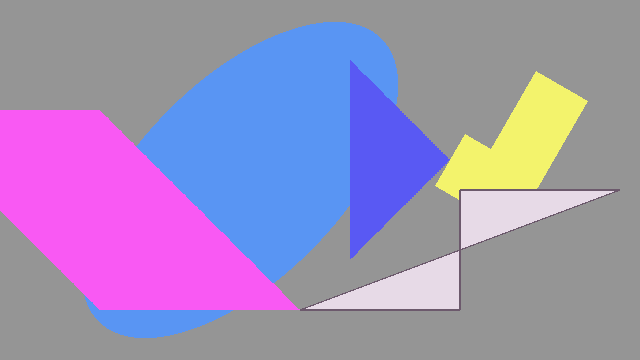
\includegraphics[width=0.5\linewidth]{imgs/hw_1_4.png}
    \caption{References for Homework 1.4.}
    \label{fig:hw1_4}
\end{figure}

\section{Keyframes Animation (10 pts)}

This part doesn't require you to write Slang code and we will use \lstinline{hw1/hw1_4.slang} to render. We will use the transformation we just learned to create some cool animations! A common way to create animation is through \emph{keyframes}. That is, we specify the state of the objects at certain time, and then \emph{interpolate} the states to fill in the inbetweening. 

For example, supposed we want to move an object from $(100, 100)$ at time $0$ to $(500, 300)$ at time $2$. To calculate the position of the object at time $1$, we simply take the average $(300, 200)$. More generally, for two keyframes at $t_0$ and $t_1$ and a time $t$ in between, we first compute
\begin{equation}
    w = \frac{t - t_0}{t_1 - t_0},
\end{equation}
and linearly interpolate the parameter $x$ using
\begin{equation}
    x(t) = (1-w) x_0 + w x_1.
\end{equation}

Our scene format specifies these keyframes using \lstinline{transform_keyframes}:
\begin{lstlisting}[language=json]
"transform_keyframes": [
    {
        "time": 0.0,
        "transform": [
            {"scale": [160, 120]},
            {"translate": [100, 50]}
        ]
    },
    {
        "time": 2.0,
        "transform": [
            {"scale": [200, 120]},
            {"translate": [300, 150]}
        ]
    },
    {
        "time": 4.0,
        "transform": [
            {"scale": [160, 120]},
            {"translate": [100, 50]}
        ]
    }
]
\end{lstlisting}

For simplicity, all the transformations inside a \lstinline{transform_keyframes} will have exactly the same types and appear in the same order.
Your job is to interpolate all of the parameters in the \lstinline{interpolate_transformation(transform_keyframes, t)} function in \lstinline{hw1_scene.py}.
Note that we are interpolating the transformation parameters directly instead of the transformation matrices (if you interpolate two rotation matrices, you may end up with something that is not a rotation matrix).

In balboa, the keyframe interpolation happens in Python on the CPU. For each frame, balboa first evaluates the transformation at the current time, constructs the corresponding transformation matrix, and computes the \lstinline{world_to_obj} matrix used by the shader. The updated shape data is then uploaded to the GPU before rendering the frame.

In a real-time renderer, we usually try to avoid re-uploading data that did not change. For example, the points of a polyline can stay on the GPU while only its transformation matrix changes every frame. Our scenes are small enough that we do not need to worry much about this optimization yet.

Test your rendering using the following commands:
\begin{lstlisting}[language=bash]
  uv run python main.py 1_5 scenes/hw1/animation.json
  uv run python main.py 1_5 scenes/hw1/sun_animation.json
  uv run python main.py 1_5 scenes/hw1/cat_animation.json
  uv run python main.py 1_5 scenes/hw1/piggy_animation.json
  uv run python main.py 1_5 scenes/hw1/pinwheel.json
  uv run python main.py 1_5 scenes/hw1/pinwheel_animation_2.json
\end{lstlisting}
We can't show animation on a PDF, so use your common sense to check the correctness!
(I had too much fun and made a lot of animations. We don't grade you on all of these.)

We will grade your results using the following scenes, using a special command that outputs an image by specifying time:
\begin{lstlisting}[language=bash]
  uv run python main.py -output outputs/hw_1_5_animation.png 1_5 -time 0.45 scenes/hw1/animation.json
  uv run python main.py -output outputs/hw_1_5_sun_animation.png 1_5 -time 0.76 scenes/hw1/sun_animation.json
  uv run python main.py -output outputs/hw_1_5_piggy_animation.png 1_5 -time 0.82 scenes/hw1/piggy_animation.json
  uv run python main.py -output outputs/hw_1_5_pinwheel_animation_2.png 1_5 -time 0.44 scenes/hw1/pinwheel_animation_2.json
\end{lstlisting}
Each worth 2.5 points.

Once this works, you should see the objects smoothly animate between the keyframes. Feel free to modify the scene and make something silly. 
One thing you may notice after things start moving is some unpleasant flickering around the boundaries of moving shapes. 
We will fix that in the next part.

\section{Antialiasing (10 pts)}
The flickering phenomenon we saw in the previous animations is called ``aliasing'' in signal processing literature (we will discuss this in depth in CSE 168). The solution to aliasing is called antialiasing. We are going to implement the simplest form of antialiasing called ``supersampling''. The idea is simple: instead of only testing/sampling the pixel center, we'll sample multiple points within a pixel, and take average between them. For this homework, we will do a $N \times N$ pattern, where $N$ is set by the parameter \lstinline{samples_per_axis} and by default it sets $N=4$. We subdivide a pixel into $N \times N$ subpixels, compute the color at the center of the subpixels, and take an average over them.

Go to \lstinline{hw1/hw1_6.slang} and implement the antialiasing scheme. Test your rendering using the following commands:
\begin{lstlisting}[language=bash]
  uv run python main.py 1_6 scenes/hw1/antialiasing.json
  uv run python main.py 1_6 scenes/hw1/animation.json
\end{lstlisting}

We show our rendering of the \lstinline{antialiasing} scene in \cref{fig:hw1_6}. We will grade your results using other scenes.

\begin{figure}[ht]
    \centering
    
\includegraphics[width=0.4\linewidth]{imgs/hw_1_6before.png}
    
\includegraphics[width=0.4\linewidth]{imgs/hw_1_6after.png}
    \caption{Without/with antialiasing.}
    \label{fig:hw1_6}
\end{figure}

We will grade your results using the following scenes:
\begin{lstlisting}[language=bash]
  uv run python main.py -output outputs/hw_1_6_antialiasing_2.png 1_6 scenes/hw1/antialiasing_2.json
  uv run python main.py -output outputs/sun_animation.png 1_6 -time 0.43 scenes/hw1/sun_animation.json
  uv run python main.py -output outputs/cat_animation.png 1_6 -time 0.87 scenes/hw1/cat_animation.json
\end{lstlisting}
The first scene is worth 5 points, whereas the other two scenes worth 2.5 points.
Try turn on/off the antialiasing by changing the \lstinline{samples_per_axis} in the scene files. Observe the difference.

\section{Alpha blending (15 pts)}
Next, let's add some transparency into the objects. Remember the RGBA thing we keep seeing? We are finally going to use the A thing. In addition to the RGB color, now each object also equips an $\alpha$ (\lstinline{alpha}) value. The lower the alpha is, the more transparent the object. $\alpha=0$ means that the object is fully transparent (so you can't see it), and $\alpha=1$ means that the object is fully opaque (so it's the same as previous parts of the homework). 

For objects with $0 < \alpha < 1$, we need to blend their colors. If there is only one object with alpha $\alpha_0$ and color $C_0$, we blend it with the background color $B$ and obtain the final color $C$ as:
\begin{equation}
C = \alpha_0 C_0 + (1 - \alpha_0) B.
\end{equation}

What if we have two objects? We can see $\alpha$ as the amount of lights captured at that layer, and $1-\alpha$ as the amount of light pass through. So for two objects with alpha $\alpha_0$, $\alpha_1$ and color $C_0$ and $C_1$, and object $0$ is in front of object $1$, we can blend them as:
\begin{equation}
C = \alpha_0 C_0 + \alpha_1 (1 - \alpha_0) C_1 + (1 - \alpha_0) (1 - \alpha_1) B.
\end{equation}

We'll let you figure out the general formula for arbitrary number of objects and turn it into code. 
Remember to compose between stroke color and fill color correctly -- they are treated as different objects.
If you are interested, \href{https://ciechanow.ski/alpha-compositing/}{here} is a great blog post talking about alpha compositing (optional reading). 
At each subpixel sample, perform normal alpha compositing of all covering fills/strokes; then average the resulting subpixel colors to obtain the pixel color.

Go to \lstinline{hw1/hw1_7.slang} and implement the alpha blending. Test your rendering using the following command:
\begin{lstlisting}[language=bash]
  uv run python main.py 1_7 scenes/hw1/alpha.json
\end{lstlisting}
We show our rendering of the \lstinline{alpha} scene in \cref{fig:hw1_7}.

\begin{figure}[ht]
    \centering
    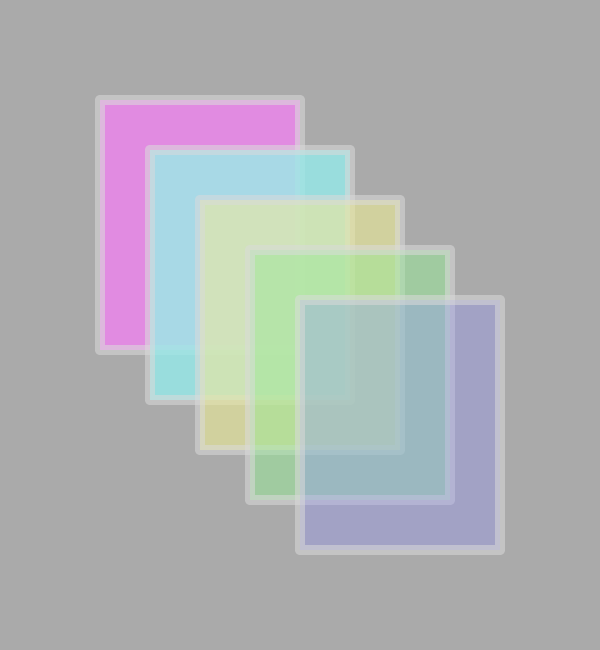
\includegraphics[width=0.5\linewidth]{imgs/hw_1_7.png}
    \caption{HW 1.7 reference.}
    \label{fig:hw1_7}
\end{figure}

We will grade your results using the following scenes:
\begin{lstlisting}[language=bash]
  uv run python main.py -output outputs/alpha_2.png 1_7 scenes/hw1/alpha_2.json
  uv run python main.py -output outputs/alpha_circles.png 1_7 scenes/hw1/alpha_circles.json
  uv run python main.py -output outputs/alpha_triangles.png 1_7 scenes/hw1/alpha_triangles.json
  uv run python main.py -output outputs/alpha_many.png 1_7 scenes/hw1/alpha_many.json
\end{lstlisting}
Each scene is worth $3.75$ points.

\section{Quadratic Bezier curves (10 pts)}
We are close to finishing! In this last part we will add one more primitive to our renderer -- the quadratic Bezier curve. This part is more mathematically involved compared to the previous parts, so don't worry too much if you could not finish everything. The implementation itself should still be fairly short; most of the challenge is figuring out what equations to solve.

A quadratic Bezier curve is defined by three control points $\mathbf{p}_0$, $\mathbf{p}_1$, and $\mathbf{p}_2$:
\begin{equation}
    \mathbf{q}(t)
    =
    (1-t)^2 \mathbf{p}_0
    + 2(1-t)t \mathbf{p}_1
    + t^2 \mathbf{p}_2,
    \qquad 0 \le t \le 1.
\end{equation}
The curve starts at $\mathbf{p}_0$, ends at $\mathbf{p}_2$, and is pulled towards $\mathbf{p}_1$ in the middle.

Similar to polylines, a quadratic Bezier curve can have a fill color and a stroke color. 
We represent a sequence of connected quadratic Bezier curves using points
\begin{equation}
    \mathbf{p}_0, \mathbf{p}_1, \mathbf{p}_2,
    \mathbf{p}_3, \mathbf{p}_4, \ldots
\end{equation}
where the first curve uses $(\mathbf{p}_0,\mathbf{p}_1,\mathbf{p}_2)$, the second curve uses $(\mathbf{p}_2,\mathbf{p}_3,\mathbf{p}_4)$, and so on. Therefore, consecutive curves share their endpoints. For a closed path $\mathbf{p}_0,\cdots,\mathbf{p}_{n-1}$, use normal segments up to $\mathbf{p}_{n-4},\mathbf{p}_{n-3},\mathbf{p}_{n-2}$, then close it using $\mathbf{p}_{2n-2},\mathbf{p}_{2n-1},\mathbf{p}_0$.

\paragraph{Fill.}
We can use almost exactly the same winding-number idea as we did for polylines. Shoot a horizontal ray from the point $\mathbf{p}$ and find all intersections between the ray and the Bezier curve.

For a quadratic Bezier curve, the $y$ coordinate of the curve is a quadratic polynomial in $t$. Therefore, finding where
\begin{equation}
    q_y(t) = p_y
\end{equation}
amounts to solving a quadratic equation.
We provide a function
\begin{lstlisting}[language=Slang]
bool solve_quadratic(float a, float b, float c, out float2 roots);
\end{lstlisting}
for you. Your job is to derive the coefficients $a$, $b$, and $c$, keep the roots inside $[0,1]$, and determine whether each intersection is on the ray. 

Remember that winding number also cares about the direction of the crossing. You can determine this by looking at whether $q_y(t)$ is increasing or decreasing at the intersection, by taking its derivative with respect to $t$.

\paragraph{Stroke.}
For the stroke, we want to find the closest point on the curve to our pixel location $\mathbf{p}$. This amounts to minimizing
\begin{equation}
    \|\mathbf{q}(t)-\mathbf{p}\|^2.
\end{equation}
At an interior minimum, its derivative with respect to $t$ should be zero:
\begin{equation}
    (\mathbf{q}(t)-\mathbf{p}) \cdot \mathbf{q}'(t) = 0.
\end{equation}
Since $\mathbf{q}(t)$ is quadratic and $\mathbf{q}'(t)$ is linear, this gives us a cubic equation.

We again provide a cubic solver (which is actually pretty hard to write, see \href{https://momentsingraphics.de/CubicRoots.html}{this page} and the referenced articles from Jim Blinn):
\begin{lstlisting}[language=Slang]
int solve_cubic(float a, float b, float c, float d,
                out float3 roots);
\end{lstlisting}
Again, your main task is to derive the coefficients that should be passed to the solver. For every valid root $t$ inside $[0,1]$, evaluate the corresponding point on the curve and check its distance to the pixel.

Our Bezier strokes have the same caps as the polyline strokes, so the way of handling them should be similar. All previous features should still apply to quadratic Bezier curves.

This probably sounds more scary than it actually is. Once you have the right polynomial coefficients, the rest of the code is quite similar to the polyline case.

Go to \lstinline{hw1/hw1_8.slang} and implement the quadratic Bezier curves. Test your rendering using the following commands:
\begin{lstlisting}[language=bash]
  uv run python main.py 1_8 scenes/hw1/smily.json
  uv run python main.py 1_8 scenes/hw1/heart.json
\end{lstlisting}
Our renderings are in \cref{fig:hw1_8}. The smily face came from \href{https://svg-tutorial.com/svg/quadratic-bezier}{this website}.

\begin{figure}[ht]
    \centering
    
\includegraphics[width=0.4\linewidth]{imgs/hw_1_8_smily.png}
    
\includegraphics[width=0.4\linewidth]{imgs/hw_1_8_heart.png}
    \caption{Homework 1.8 references.}
    \label{fig:hw1_8}
\end{figure}

We will grade you using the following scenes (try seeing the full animation first!)
\begin{lstlisting}[language=bash]
  uv run python main.py -output outputs/hw_1_8_test_card.png 1_8 scenes/hw1/test_card.json
  uv run python main.py -output outputs/hw_1_8_flower.png 1_8 scenes/hw1/flower.json
  uv run python main.py -output outputs/hw_1_8_jellyfish.png 1_8 -time 0.91 scenes/hw1/jellyfish.json
\end{lstlisting}

\section{Design your own scenes (5 pts)}

One last stretch! Design a scene yourself and submit the scene and your rendering/animation to us.
Only completion is graded.

\end{document}